%\begin{figure}[h]
%	\centering\includegraphics[width=0.8\textwidth]{fig/figure_4}
%	\caption{Extrem coole Grafik!}
%\end{figure}


% SUBFIGURE
%\begin{figure}[h]
%	\centering
%	\subfigure[]{\includegraphics[width=0.49\textwidth]{fig/2_a_plot}}
%	\subfigure[]{\includegraphics[width=0.49\textwidth]{fig/2_b_plot}}
%	\caption{\textbf{a)} Temperatur des Aluminium Hohlzylinders gegen die Zeit aufgetragen, \textbf{b)} Änderung der Temperatur gegenüber der Temperatur aufgetragen. Jeweils unter Verwendung des Heizdrahtes.}
%	\label{fig:2_1_plot}
%\end{figure}

\section{Kalibrierung des Röntgendetektors}

Der Versuch wird wie in der Vorbereitung beschrieben durchgeführt.
Dabei konnte kein Nutzen durch die Verwendung einer höheren Verstärkungsstufe beobachtet werden, die K$_\alpha$ und K$_\beta$-Linien der Standardproben ließen sich auch bei V = 4 nicht klar voneinander unterscheiden. Die Kalibrierung wird daher auch nur anhand der K$_\alpha$-Linien durchgeführt.\\
Einzige Ausnahme bildet Silber, bei welchem im Röntgenspektrum zwei klar erkennbare Peaks vorhanden waren. Diese lagen allerdings in einem so hohen Energiebereich, dass sie mit einer Verstärkung von V = 4 nicht mehr auf der Skala gewesen wären.\\
Bei Blei handelt es sich außerdem um die L$_\alpha$ und L$_\beta$-Linie, da die K$_\alpha$-Linie deutlich höher als die maximal erreichbaren 35\;keV liegt.\\
Die gefitteten Peaks der einzelnen Proben befinden sich in Tabelle \ref{tab:a1_peaks}.

\xtable{htb}{a1_peaks}{Messwerte der Fits unterschiedlicher Röntgenspektren}{(Aufg. 1)}

Die Gleichung der mit Hilfe von QtiPlot an die Messwerte gefitteten Gerade (s. Abb. \ref{fig:a1_fit}) inkl. statistischer Fehler sieht folgendermaßen aus:
\begin{equation}
	E(K) = (0,00807\pm 0,00002)K\cdot\si{\kilo\electronvolt} + (1,40\pm 0,04)\cdot\si{\kilo\electronvolt}
\end{equation}

\begin{figure}[h]
	\centering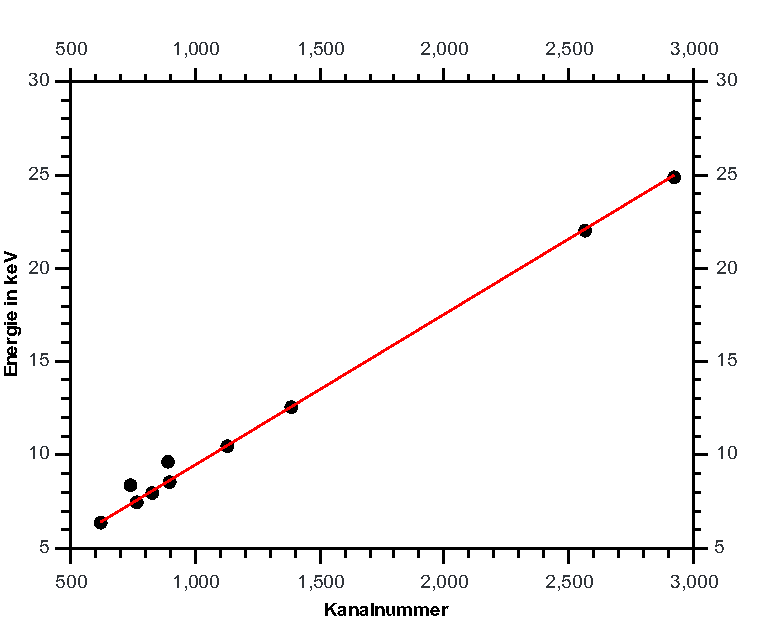
\includegraphics[width=0.8\textwidth]{fig/a1_fit}
	\caption{Skalierungsgerade zur Eichung des Röntgendetektors.}
	\label{fig:a1_fit}
\end{figure}

Es ist zu erkennen, dass die Messwerte der Röntgenstrahlung ohne Materialprobe als einzige von der Geraden abweichen und die Regression bei niedrigeren Kanalnummern nach oben ziehen. Dies liegt daran, dass die Zählrate in diesem Versuchsteil zu hoch war und der VKA somit überfordert wurde. Die Messwerte sind daher in Abb. \ref{fig:a1_fit} aufgeführt, wurden aber für die lineare Regression nicht verwendet.

\section{Bestimmung der Energieauflösung des RED}